\documentclass[11pt]{article}
\usepackage[utf8]{inputenc}
\usepackage[ngerman]{babel}

\usepackage{amsmath,amsthm,amssymb,amsfonts}

\usepackage{graphicx}
\graphicspath{{abb/}}
\usepackage{float}
\usepackage{tikz}

\usepackage{fancyhdr} % For headers and footers
\usepackage{geometry}
\usepackage{listings}
\usepackage{hyperref}
\hypersetup{
    linkcolor=blue,     
    urlcolor=cyan,
}

\geometry{
    a4paper, % Change this if you intend to print on a different paper size, such as letter paper.
    left=20mm,
    right=20mm,
    top=30mm,
    bottom=30mm,
}

\title{Dynamik - Energie}
\author{Emil Staikov}
\date{10. Mai 2021}

\begin{document}
\maketitle

\section{Arbeit}
Wenn sich ein Objekt über einen Weg $\vec{s}$ bewegt, und dabei eine Kraft $\vec{F}$ auf dieses Objekt wirkt, so wird an dem Objekt Arbeit $W$ verrichtet. Wir definieren die Arbeit $W$ für konstante Kräfte als das Produkt aus der parallel zum Weg wirkenden Kraft und der Länge des Wegs, also 
\begin{equation*}
    W = |\vec{F}||\vec{s}|\cos \alpha
\end{equation*}
wobei $\alpha$ der Winkel zwischen Weg und wirkender Kraft ist.
\begin{figure}[H]
    \centering
    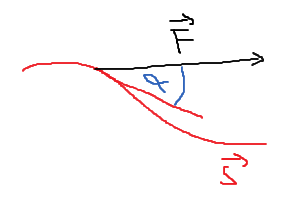
\includegraphics[width=0.3\textwidth]{arbeit-def.png}
\end{figure}
Dabei fällt uns auf, dass wir in Abhängigkeit von der Größe des Winkels einige Fälle unterscheiden können: 
\begin{itemize}
    \item $\alpha < 90$°, also die Kraft wirkt in Richtung des Wegs: $1 \geq \cos\alpha > 0$, also $W > 0$
    \item $\alpha = 90$°, also die Kraft wirkt senkrecht zum Weg: $\cos\alpha = 0$, also $W = 0$
    \item $\alpha > 90$°, also die Kraft wirkt entgegen der Richtung des Wegs: $0 > \cos\alpha \geq -1$, also $W < 0$
\end{itemize}
Die Einheit der Arbeit ist $[W] = \frac{kg\cdot m^2}{s^2} = Nm = J$, wobei $J$ für die Einheit Joule steht. 

\section{Leistung}
Wir definieren die Leistung $P$ als verrichtete Arbeit pro Zeiteinheit, also 
\begin{equation*}
    P = \frac{\Delta W}{\Delta t}
\end{equation*}
Die Einheit der Leistung ist $[P] = \frac{J}{s} = W$, wobei $W$ für die Einheit Watt steht. 

\section{Energie}
\subsection{Zusammenhang von Arbeit und kinetischer Energie}
Wenn wir über ein Zeitintervall $\Delta t$ eine Kraft $F$ parallel zur Bewegungsrichtung eines Körpers ausüben, so verändert sich seine Geschwindigkeit von $v_0$ zu $v$. Das haben wir bis jetzt mithilfe der Newton'schen Axiome modelliert und untersucht. Uns fällt jedoch auf, dass wir in diesem Prozess an dem Körper ebenfalls Arbeit verrichten. Im folgenden schließen wir auf die Verbindung zwischen verrichteter Arbeit und Geschwindigkeitsänderung. Wir betrachten alle Größen als Skalare, da wir nur den Fall paraller Kräfte und Wege betrachten. 
\begin{align*}
    W &= Fs = mas \\
    &= m \frac{(v - v_0)}{\Delta t}\frac{(v + v_0) \Delta t}{2} \quad (*) \\
    &= m\frac{v^2 - v_0^2}{2} \\
    &= \frac{1}{2}mv^2 - \frac{1}{2}mv_0^2
\end{align*}
Zu $(*)$: Wir verwenden hier die Definition der Beschleunigung, sowie die Tatsache, dass $s$ der Fläche unter dem Graphen von $v$ entspricht. Diese Fläche können wir für linear wachsende Geschwindigkeiten, also $a = const.$ bzw. $F = const.$, wie oben ausdrücken. Genauer betrachtet wird das in der Herleitung der Formel für $s(t)$ im Fall konstanter Beschleunigung.  \\\\
Die Größe $\frac{1}{2}mv^2$ definieren wir nun als kinetische Energie $E_{kin}$ eines Körpers der Masse $m$, der sich mit Geschwindigkeit $v$ bewegt. Die kinetische Energie ist ein Skalar, also eine Zahl, nicht ein Vektor, und hat ebenfalls die Einheit $J$ (Joule). Die kinetische Energie hängt mit der verrichteten Arbeit nach der eben getätigten Herleitung wie folgt zusammen: 
\begin{equation*}
    W = \Delta E_{kin}
\end{equation*}

\subsection{Potentielle Energie}
Wir bemerken, dass beim Heben eines Objekts in der Nähe der Erde auch Arbeit verrichtet wird - wir heben ein Objekt durch eine bestimmte Höhe, während die Gravitationskraft wirkt - ohne, dass sich die Geschwindigkeit des Objekts ändert. Ähnlich verhält es sich mit Objekten an Federn - wenn wir die Feder zusammendrücken, bewegen wir das Objekt durch einen Weg, und die Federkraft wirkt entlang dieses Wegs, aber die Geschwindigkeit des Objekts am Anfang und am Ende des Zusammenschiebens sind gleich. Zusätzlich beobachten wir, dass wenn ein Objekt aus einer Höhe herunterfällt, es eine bestimmte Geschwindigkeit erlangt, und das eine Feder beim Ausdehnen bzw. Zusammenziehen dem daran hängenden Objekt ebenfalls eine Geschwindigkeit verleiht. \\\\ 
Um dies erfassen zu können, definieren wir jetzt eine weitere Art der Energie, die mit der Lage von Objekten in einem System zusammenhängt. Wir nennen diese Art \textbf{potentielle Energie}. Für alle interessierten: Wir definieren potentielle Energien nur für sogenannte \textbf{konservativen Kräften}, zu denen z.B. die Reibung nicht gehört. Um diese korrekt zu definieren, bräuchten wir jedoch ein genaueres Verständnis von Arbeit. \\\\
Wir definieren die Änderung in potentieller Energie bezüglich einer Kraft wie folgt: 
\begin{equation*}
    -W = \Delta E_{pot}
\end{equation*}
Dabei fällt auf, dass 
\begin{equation*}
    -W = -F\Delta s = \Delta E_{pot} \\
    \iff F = - \frac{\Delta E_{pot}}{\Delta s}
\end{equation*}
Also die negative Änderung der potentiellen Energie mit dem Ort gleich der Kraft ist. Die Einheit der potentiellen Energie ist natürlich erneut $J$ (Joule).

\subsubsection{Potentielle Energie der Gravitation}
In der Nähe der Erde wirkt die Gravitationskraft $F = mg$ senkrecht nach unten. Wenn wir ein Objekt von der Höhe $h_0$ auf die Höhe $h$ heben, so verrichten wir an dem Objekt die folgende Arbeit: 
\begin{equation*}
    W = Fs = mg(h_0 - h)
\end{equation*} 
Dabei wird beim Heben ($h > h_0$) negative Arbeit und beim Fall positive Arbeit ($h < h_0$) verrichtet. Für die Änderung der potentiellen Energie gilt dann: 
\begin{equation*}
    \Delta E_{pot} = -W = -mg(h_0 - h) = mgh - mgh_0
\end{equation*}
Dabei erhöht sich beim Heben die potentielle Energie, und sie sinkt beim erneuten Herabfallen. Da wir uns nur für die Änderung der potentiellen Energie interessieren, können wir $h_0$ beliebig wählen, und die potentielle Energie für dieses $h_0$ zu null bestimmen. Meistens wählen wir den Boden, also die Starthöhe. 

\subsubsection{Potentielle Energie der Feder}
Die Federkraft $F_D$ wirkt nach dem Hooke'schen Gesetz $F_D = -D \Delta x$, wobei $\Delta x$ die Auslenkung und $D$ die Federkonstante ist, stets entgegen der Auslenkung der Feder. Wenn wir also eine Feder auslenken, verrichten wir stets die negative Arbeit 
\begin{equation*}
    W = F_D\Delta x = - D (\Delta x) ^2
\end{equation*}
Die potentielle Energie der Feder ist dann im Gegenzug stets positiv, und gegeben durch 
\begin{equation*}
    \Delta E_{pot} = -W = D (\Delta x) ^2
\end{equation*}
Wir haben hier schon implizit einen Nullpunkt für die potentielle Energie gewählt. Sie ist in der Ruhelage der Feder, also für $\Delta x = 0$, null. 

\subsection{Energieerhaltung}
Wir haben bereits einige Situationen beschrieben, in denen potentielle Energie in kinetische Energie und kinetische in potentielle Energie umgewandelt wird. Wir können sogar noch weiter gehen: In Systemen, in denen nur Kräfte wirken, mit denen wir eine potentielle Energie verbinden können, und an denen keine Arbeit von außen verrichtet wird, bleibt die Energie erhalten. Wenn die kinetische Energie des Systems kleiner wird, können wir sie als potentielle Energie wiederfinden, und andersherum:
\begin{gather*}
    W = \Delta E_{kin} \land -W = \Delta E_{pot} \\
    \Delta E_{kin} = -\Delta E_{pot} \iff \Delta E_{kin} + \Delta E_{pot} = 0 
\end{gather*}
Die meisten Systeme, die wir behandeln werden, erfüllen diese Bedingung. Eine wichtige Ausnahme sind inelastische Stöße, diese werden wir später noch genauer betrachten. Als teaser: Es gibt noch andere Formen von Energie, z. B. Wärme. Wärme entsteht z. B. bei Reibung oder Verformung von Körpern, wenn in unserem System Sachen aneinander Reiben oder sich Verformen, geht ein Teil der potentiellen oder kinetischen Energie in die Wärme über. Dann gilt zwar immernoch in gewissem Sinn die Energieerhaltung, aber wir müssen noch mehr Arten der Energie betrachten. Dies ist in den meisten Fällen nicht sinnvoll zu modellieren, daher können wir in solchen Fällen nicht mehr mit Energieerhaltung rechnen. 

\subsubsection{Ein Beispiel}
Wir betrachten wieder unseren altbekannten senkrechten Wurf. Wenn wir einen Stift der Masse $m = 50g$ mit einer Geschwindigkeit von $v = 10 \frac{m}{s}$ hochwerfen, wie hoch wird er fliegen? \\\\
Die Energie $E$ des Systems direkt nach dem Hochwerfen ist genau die kinetische Energie des Stifts. 
\begin{equation*}
    E = \frac{1}{2}mv^2 = \frac{1}{2}0.05kg\cdot (10 \frac{m}{s})^2 = 2.5 \frac{kg\cdot m^2}{s^2} = 2.5 J
\end{equation*}
Wenn die maximale Höhe $h$ erreicht ist, hat der Stift keine Geschwindigkeit mehr, da sich seine Bewegungsrichtung gerade dort umdreht. Damit ist seine kinetische Energie ebenfalls $0$, und die gesamte Energie des Stifts ist die potentielle Energie seiner Höhe. Wir vernachlässigen die Reibung zwischen Luft und Stift, folglich sind die einzigen auf den Stift wirkenden Kräfte Gravitation, sowie die Kraft zwischen Hand und Stift und die Gegenkraft zwischen Stift und Hand beim Hochwerfen. Mit der Gravitation können wir eine potentielle Energie assoziieren, und die beiden anderen Kräfte verrichten an dem Stift entgegengesetzt gleiche Arbeit, folglich ist die gesamte an dem Stift von außen verrichtete Arbeit $0$. Damit bleibt die Energie des Stifts erhalten, und wir können die maximale Höhe, die der Stift erreicht, ermitteln: 
\begin{gather*}
    E = 2.5 J = mgh = 0.05kg \cdot 9.8 \frac{m}{s^2} \cdot h \\
    \iff h = \frac{2.5 J}{0.05kg \cdot 9.8 \frac{m}{s^2}} = \frac{2.5J}{0.05 \cdot 9.8} \frac{\frac{kg\cdot m^2}{s^2}}{kg\cdot\frac{m}{s^2}} \approx 5.1 m
\end{gather*}

\end{document}